\documentclass[12pt]{article}

\usepackage[utf8x]{inputenc}
\usepackage[L7x, T2A]{fontenc}
\usepackage[lithuanian]{babel}
\usepackage{vwcol}  
\usepackage{sectsty}
\usepackage{setspace}
\usepackage{fancyhdr}
\usepackage{graphicx}
\usepackage{ragged2e}
\usepackage{titlesec}
\usepackage{epsfig}
\usepackage{indentfirst}
\usepackage[top=2cm, bottom=2cm, left=3cm, right=1.5cm]{geometry}
\usepackage{makecell}
\usepackage[justification=centering]{caption}
\usepackage{titlesec}
\usepackage{fullpage}
\usepackage{amsmath,amssymb,amsthm,enumitem}
\usepackage{enumitem}
\usepackage{color}  
\usepackage[hypertexnames=false]{hyperref}
\hypersetup{
    colorlinks=true,
    linktoc=all,
    linkcolor=black,
}
\usepackage[tocindentauto]{tocstyle}
\usetocstyle{standard}

\usepackage{svg}

\makeatletter
\expandafter\let\csname L7x-cmd\endcsname\@changed@cmd
\makeatother

\addto\extraspolish{\fontencoding{L7x}\selectfont}
\addto\noextraspolish{\fontencoding{\encodingdefault}\selectfont}

\setlength\parindent{1cm}

\title{VILNIAUS UNIVERSITETAS \\
MATEMATIKOS IR INFORMATIKOS FAKULTETAS \\
PROGRAMŲ SISTEMŲ KATEDRA}
\author{}
\date{}

\pagestyle{fancy}
\fancyhead{}
\fancyfoot{}
\fancyfoot[R]{\thepage}
\renewcommand{\headrulewidth}{0pt}
\renewcommand{\baselinestretch}{1.5}


\renewcommand{\thesubsection}{FR\arabic{subsection}}
\renewcommand*{\theenumi}{\thesubsection.\arabic{enumi}}
\renewcommand*{\theenumii}{\thesubsubsection.\theenumi.\arabic{enumii}}

%\titleformat{\subsection}{\Large\bfseries}{\arabic{subsection}}{1em}{}
\titleformat{\subsubsection}{\bfseries}{\thesubsection.\arabic{subsubsection}}{1em}{}

\begin{document}
	\clearpage
	\maketitle
	\thispagestyle{empty}

	\bigbreak
	\bigbreak
	\bigbreak
	\bigbreak

	\begin{center}
		\begin{Large}
			\textbf{Transporto priemonių skelbimų aplikacija} \\
		\end{Large}
		\begin{large}
			\textbf{Application for Vehicle Advertisement} \\
		\end{large}
		Programų sistemų inžinerijos I laboratorinis darbas Nr. 2 \\

		\bigbreak
		\bigbreak
		\bigbreak
		\bigbreak
		\bigbreak
		\bigbreak
		\bigbreak
		\bigbreak
		\bigbreak

		\begin{tabular}{ll}
			Atliko:        & 2 kurso 5 grupės studentai \\
		               	   & Toma Burneikaitė \\
		               	   & Žygimantas Stongvilas \\
		                   & Mantas Jurčius \\
		                   & Rimvydas Meškauskas \\
			Darbo vadovas: & asist., dr. Vytautas Valaitis
		\end{tabular}

		\bigbreak
		\bigbreak
		\bigbreak
		\bigbreak
		\bigbreak
		\bigbreak
		\bigbreak
		\bigbreak
		\bigbreak

		Vilnius - 2018
	\end{center}
	\pagebreak
	
	\renewcommand{\baselinestretch}{0.5}
	\tableofcontents
	\renewcommand{\baselinestretch}{1.5}
	\pagebreak	
	
	\section*{Įvadas}	
	\addcontentsline{toc}{section}{Įvadas}	
	
	Šiame projektiniame darbe pristatomas transporto priemonių skelbimų programėlės „AutoINF“ įgyvendinimas. Mūsų vizija yra pasaulis, kuriame kiekvienas žmogus gali greitai, paprastai ir be vargo rasti reikiamą transporto priemonę, nesvarbu, kokiame Europos krašte ji bebūtų. Siekdami to mes užsibrėžiame tikslą sukurti mobiliesiems įrenginiams skirtą programėlę, kuri leistų pasiekti transporto priemonių skelbimus iš visos Europos. Idėja kilo todėl, kad dabar įvairių transporto priemonių skelbimai yra daugybėje skirtingų puslapių (šaltinių) ir norint susirasti naudingiausią pasiūlymą dažniausiai reikia pereiti per daugiau nei vieną puslapį. „AutoINF“ projekto tikslas yra sukurti programėlę, kuri supaprastintų transporto priemonių ieškojimo procesą ir padėtų vartotojui sutaupyti laiko tą darant, surinkdama visus skelbimus iš populiariausių Europos transporto priemonių skelbimų puslapių pagal vartotojo nurodytus kriterijus. Taip pat norima, kad programėle būtų paprasta naudotis ir kad ši programėlė sugebėtų pateikti kuo daugiau vartotojui aktualios informacijos apie tai, ko jis ieško.
	\pagebreak
	
	\section*{Funkciniai reikalavimai}
	\addcontentsline{toc}{section}{Funkciniai reikalavimai}
	
	\subsection{Bendri reikalavimai}
	\begin{enumerate}[labelindent=10pt,leftmargin=2.2cm]
		\item Įrenginys, kuriame naudojama programinė sistema, turi turėti prieigą prie interneto.
		\item Programinės įrangos įdiegimas laisvai prieinamas visiems norintiems ja naudotis.
		\item Vartotojas turi galimybę keisti savo asmeninius duomenis (vartotojo vardą, el. paštą bei slaptažodį).
		%\item Kiekvieno vartotojo skelbimai, pridėti prie jo mėgstamiausių sąrašo, yra saugomi vartotojo įrenginyje.
		\item Valiutų kursai nustatomi remiantis Lietuvos Banko duomenimis.
		\item Sistema vartotojui neprisijungus leidžia atlikti jos pagrindinę funkciją (skelbimų paieška).
		\item Sistema vartotojui prisijungus leidžia atlikti pagrindinę funkciją (skelbimų paieška) ir papildomą funkciją (skelbimų saugojimas mėgstamiausių sąraše).
		\item Mėgstamiausių sąrašas kiekvienam vartotojui yra prieinamas tik jam ir niekam kitam.
		%\item Sistema vartotojui leidžia iš bet kurio jos lango grįžti į pagrindinį langą.
	\end{enumerate}
	\pagebreak
	
	\renewcommand*{\theenumi}{\thesubsubsection.\arabic{enumi}}
	\renewcommand*{\theenumii}{\thesubsubsection.\theenumi.\arabic{enumii}}
	\renewcommand*{\theenumiii}{\thesubsubsection.\theenumi.\theenumii.\arabic{enumiii}}
	\subsection{Vartotojo užduočių reikalavimai}\label{Vartotojo_reikalavimai}
	Šiame skyriuje nagrinėjami vartotojui aktualūs reikalavimai sistemai „AutoINF“. Pateikiami vartotojo funkciniai reikalavimai, užduočių scenarijai bei jų plėtiniai.
	
	\begin{figure}[h]
		\begin{center}
			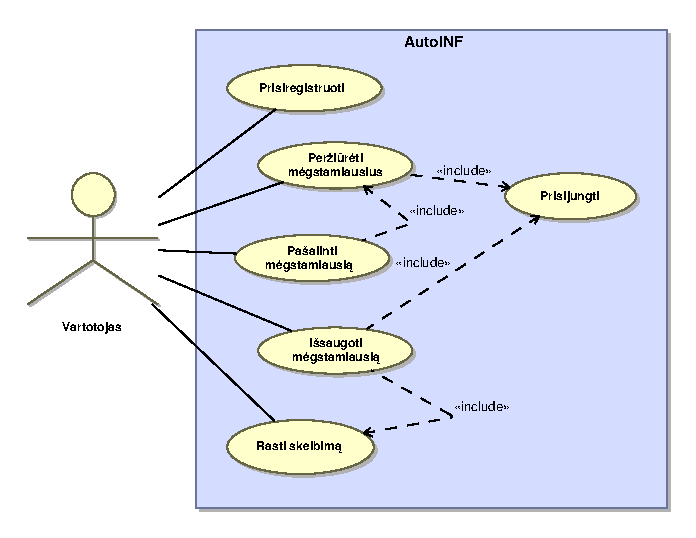
\includegraphics[width=0.7\textwidth]{TikslaiVartotojas.eps}
			\caption{Sistemos užduočių diagrama iš vartotojo perspektyvos\label{UseCaseUser}}
		\end{center}
	\end{figure}
	\pagebreak
	
	\subsubsection{Pagrindinio meniu reikalavimai}
	\begin{enumerate}[labelindent=10pt,leftmargin=2.2cm]
		\item Pagrindiniame lange vartotojas, jei jis neprisijungęs, turi galimybę pasinaudoti šiomis sistemos funkcijomis: prisiregistruoti, prisijungti bei ieškoti skelbimų.
	\end{enumerate}
		
		\begin{center}
		\captionof{table}{Pagrindinio lango scenarijus, kai vartotojas nėra prisijungęs\label{UserNotLoggedIn}}
		\begin{tabular}{ | c | c | c | }
			\hline
			Žingsnis & Aktorius   & Veiklos apibūdinimas \\ \hline
			1        & Aplikacija & \makecell{Paprašo pasirinkti norimą veiksmą: \\ Prisiregistruoti \\ Prisijungti \\ Rasti skelbimą} \\ \hline
			2        & Vartotojas & Pasirenka veiksmą \\ \hline
			3        & Aplikacija & Įvykdo pasirinktą veiksmą \\ \hline
		\end{tabular}
		\bigskip
		\end{center}
		
	\begin{enumerate}[resume, labelindent=10pt,leftmargin=2.2cm]
		\item Pagrindiniame lange vartotojas, jei jis prisijungęs, turi galimybę pasinaudoti šiomis sistemos funkcijomis: ieškoti skelbimų, peržiūrėti mėgstamiausius.
	\end{enumerate}
		
		\begin{center}
		\captionof{table}{Pagrindinio lango scenarijus, kai vartotojas yra prisijungęs\label{UserLoggedIn}}		
		\begin{tabular}{ | c | c | c | }
			\hline
			Žingsnis & Aktorius   & Veiklos apibūdinimas \\ \hline
			1        & Aplikacija & \makecell{Paprašo pasirinkti norimą veiksmą: \\ Peržiūrėti mėgstamiausius \\ Pašalinti mėgstamiausią \\ Išsaugoti mėgstamiausią \\ Rasti skelbimą} \\ \hline
			2        & Vartotojas & Pasirenka veiksmą \\ \hline
			3        & Aplikacija & Įvykdo pasirinktą veiksmą \\ \hline
		\end{tabular}
		\end{center}		
	\pagebreak
	
	\subsubsection{Vartotojo registracijos reikalavimai}
	\begin{enumerate}[labelindent=10pt,leftmargin=2.2cm]
		\item Sėkmingos registracijos atveju sistema vykdo \ref{UserRegScen} lentelėje nurodytą veiksmų seką.
	\end{enumerate}
		
		\begin{center}
		\captionof{table}{Vartotojo registracijos pagrindinis scenarijus\label{UserRegScen}}		
		\begin{tabular}{ | c | c | c | }
			\hline
			Žingsnis & Aktorius     & Veiklos apibūdinimas \\ \hline
			1        & Vartotojas   & Pasirenka registraciją \\ \hline
			2        & Aplikacija   & Atidaro registracijos langą \\ \hline
			3        & Vartotojas   & \makecell{Suveda prisiregistravimo duomenis ir \\ spaudžia mygtuką „Prisiregistruoti“} \\ \hline
			4        & Aplikacija   & Validuoja duomenis ir siunčia užklausą į serverį \\ \hline
			5        & Serveris     & Siunčia užklausą į duomenų bazę \\ \hline
			6        & Duomenų bazė & \makecell{Išsaugo naujos paskyros duomenis ir \\ perspėja serverį apie sėkmingą registraciją} \\ \hline
			7        & Serveris     & Perspėja aplikaciją apie sėkmingą registraciją \\ \hline
			8        & Aplikacija   & \makecell{Parodo pranešimą apie registracijos sėkmingumą, \\ perkrauna pagrindinį langą su prisijungusio vartotojo \\ interfeisu ir laukia, kol vartotojas atliks kitą veiksmą} \\ \hline
		\end{tabular}
		\end{center}
		\bigskip
		
	\begin{enumerate}[resume, labelindent=10pt,leftmargin=2.2cm]
		\item Nesėkmingos registracijos atveju sistema į klaidas reaguoja pagal \ref{UserRegScenExtra} lentelę.
	\end{enumerate}
		
		\begin{center}
		\captionof{table}{Vartotojo registracijos scenarijaus plėtiniai\label{UserRegScenExtra}}		
		\begin{tabular}{ | c | c | c | }
			\hline
			Žingsnis & Sąlyga & Veiklos apibūdinimas \\ \hline
			4a       & \makecell{Vartotojo duomenų \\ validacija nesėkminga} & \makecell{Klaidingai užpildyti (neužpildyti) laukai yra paryškinami \\ raudonai ir lango viršuje parodomas tekstas, kad kai \\ kurie laukai yra užpildyti klaidingai (neužpildyti)} \\ \hline
			6a       & \makecell{Duomenų bazėje \\ nepavyko išsaugoti \\ duomenų} & Parodomas pranešimas apie nesėkmingą registraciją \\ \hline
		\end{tabular}
		\end{center}
		\pagebreak
		
	\begin{enumerate}[resume, labelindent=10pt,leftmargin=2.2cm]
		\item\label{Validation} Vartotojui patvirtinus registraciją sistema turi validuoti vartotojo įvestus duomenis:
		
		\begin{enumerate}[label=\theenumi.\arabic{enumii}]
			\item Visi privalomi laukai (vartotojo vardas, el. paštas bei slaptažodis) turi būti užpildyti.
			\item Galimi simboliai: lotyniškos mažosios bei didžiosios raidės, skaičiai.
			\item El. pašto lauko įvestis turi būti formato „pavyzdys@mail.lt“.
			\item Slaptažodį turi sudaryti bent 8 simboliai, tarp kurių yra bent viena mažoji raidė, didžioji raidė ir bent vienas skaičius.
		\end{enumerate}	
		
		\item Prieš sukurdama naują paskyrą sistema turi užtikrinti, kad dar neegzistuoja paskyra su įvestu vartotojo vardu ar el. paštu.
		\item Vartotojo vardas ir el. paštas duomenų bazėje saugomi simbolių eilutės („string“) formatu, o slaptažodžiui pritaikoma maišos („hash“) funkcija.
	\end{enumerate}	
	\pagebreak
	
	\subsubsection{Vartotojo prisijungimo reikalavimai\label{LogInLabel}}
	\begin{enumerate}[labelindent=10pt,leftmargin=2.2cm]
		\item Sėkmingo prisijungimo atveju sistema vykdo \ref{UserLogInScen} lentelėje nurodytą veiksmų seką.
	\end{enumerate}
		
		\begin{center}
		\captionof{table}{Vartotojo prisijungimo pagrindinis scenarijus\label{UserLogInScen}}		
		\begin{tabular}{ | c | c | c | }
			\hline
			Žingsnis & Aktorius     & Veiklos apibūdinimas \\ \hline
			1        & Vartotojas   & Pasirenka prisijungimo funkciją \\ \hline
			2        & Aplikacija   & Parodo prisijungimo langą \\ \hline
			3        & Vartotojas   & \makecell{Įveda prisijungimo duomenis ir \\ spaudžia mygtuką „Prisijungti“} \\ \hline
			4        & Aplikacija   & Validuoja duomenis ir siunčia užklausą į serverį \\ \hline
			5        & Serveris     & Siunčia užklausą į duomenų bazę \\ \hline
			6        & Duomenų bazė & \makecell{Patikrina, ar tokia paskyra egzistuoja ir \\ praneša serveriui apie sėkmingą prisijungimą} \\ \hline
			7        & Serveris     & Praneša aplikacijai apie sėkmingą prisijungimą \\ \hline
			8        & Aplikacija   & \makecell{Parodo pagrindinį langą su papildomomis \\ prisijungusio vartotojo funkcijomis} \\ \hline
		\end{tabular}
		\bigskip
		\end{center}
		
	\begin{enumerate}[resume, labelindent=10pt,leftmargin=2.2cm]
		\item Nesėkmingo prisijungimo atveju sistema į klaidas reaguoja pagal \ref{UserLogInScenExtra} lentelę.
	\end{enumerate}		
		
		\begin{center}
		\captionof{table}{Vartotojo prisijungimo scenarijaus plėtiniai\label{UserLogInScenExtra}}		
		\begin{tabular}{ | c | c | c | }
			\hline
			Žingsnis & Sąlyga & Veiklos apibūdinimas \\ \hline
			4a       & \makecell{Įvestų duomenų \\ validacija nesėkminga} & \makecell{Klaidingai užpildyti (neužpildyti) laukai yra paryškinami \\ raudonai ir lango viršuje parodomas tekstas, kad kai \\ kurie laukai yra užpildyti klaidingai (neužpildyti)} \\ \hline
			6a       & \makecell{Suvesti klaidingi \\ prisijungimo duomenys} & \makecell{Parodomas pranešimas apie paskyros \\ neegzistavimą / klaidingą slaptažodį} \\ \hline
		\end{tabular}
		\end{center}
	\pagebreak
	
	\begin{enumerate}[resume, labelindent=10pt,leftmargin=2.2cm]
		\item Prisijungimo duomenų validacija tokia pati kaip ir \ref{Validation} punkte nurodyta registracijos metu vykdoma validacija (išskyrus prisijungimui nenaudojamą el. paštą).
		\item Slaptažodis lyginamas su rastos paskyros slaptažodžiu iš pradžių pritaikius maišos („hash“) funkciją.
	\end{enumerate}
	\pagebreak
	
	\subsubsection{Vartotojo skelbimų paieškos reikalavimai}
	\begin{enumerate}[labelindent=10pt,leftmargin=2.2cm]
		\item Sėkmingos paieškos atveju sistema vykdo \ref{UserSearchScen} lentelėje nurodytą veiksmų seką.
	\end{enumerate}
		
		\begin{center}
		\captionof{table}{Vartotojo skelbimų ieškojimo pagrindinis scenarijus\label{UserSearchScen}}		
		\begin{tabular}{ | c | c | c | }
			\hline
			Žingsnis & Aktorius     & Veiklos apibūdinimas \\ \hline
			1        & Vartotojas   & \makecell{Vartotojas įveda paieškos kriterijus \\ ir spaudžia mygtuką „Ieškoti“} \\ \hline
			2        & Aplikacija   & Siunčia užklausą į serverį \\ \hline
			3        & Serveris     & Siunčia užklausą į paieškos modulį \\ \hline
			4        & Paieškos modulis & \makecell{Randa skelbimus, atitinkančius vartotojo \\ nurodytus kriterijus ir grąžina juos serveriui} \\ \hline
			5        & Serveris     & Grąžina aplikacijai rastus skelbimus  \\ \hline
			6        & Aplikacija   & Parodo rastų skelbimų sąrašą \\ \hline
			7        & Vartotojas   & Paspausžia ant skelbimo \\ \hline
			8        & Aplikacija   & Atidaro skelbimo langą \\ \hline
		\end{tabular}
		\end{center}
		\bigskip

	\begin{enumerate}[resume,labelindent=10pt,leftmargin=2.2cm]
		\item Nesėkmingos paieškos atveju sistema į klaidas reaguoja pagal \ref{UserSearchScenExtra} lentelę.
	\end{enumerate}

		\begin{center}
		\captionof{table}{Vartotojo skelbimų ieškojimo scenarijaus plėtiniai\label{UserSearchScenExtra}}		
		\begin{tabular}{ | c | c | c | }
			\hline
			Žingsnis & Sąlyga & Veiklos apibūdinimas \\ \hline
			1a       & \makecell{Vartotojas nesuveda \\ privalomų paieškos kriterijų} & \makecell{Vartotojas įspėjamas, kad negalima \\ palikti neužpildytų privalomų laukų} \\ \hline
			5a       & Nerasta skelbimų & \makecell{Parodomas pranešimas, kad nėra skelbimų, \\ atitinkančių nurodytą filtrą, ir vartotojas yra \\ grąžinamas į pagrindinį (paieškos) langą } \\ \hline
			7a       & \makecell{Vartotojas nepaspaudžia \\ ant skelbimo} & \makecell{Aplikacija laukia, kol bus paspausta ant \\ skelbimo arba kol vartotojas ieškos naujų \\ skelbimų pagal kitą filtrą} \\ \hline
		\end{tabular}
		\end{center}
		\pagebreak
		
	\begin{enumerate}[resume,labelindent=10pt,leftmargin=2.2cm]
		\item Pradėdama paiešką sistema filtruoja skelbimų šaltinius:
		
		\begin{enumerate}[label=\theenumi.\arabic{enumii}]
			\item Jei nurodyti ieškomų transporto priemonių tipai, imami tik tie šaltiniai, kuriuose yra šių tipų transporto priemonių skelbimai.
			\item Jei nurodytos valstybės, imami tik tie šaltiniai, kuriuose talpinami tose valstybėse skelbiamų transporto priemonių skelbimai.
		\end{enumerate}				
		
		\item Ieškodama skelbimų, sistema iš kiekvieno tinkančio skelbimų šaltinio gauna visus skelbimus ir rodo tik tuos, kurie atitinka visus vartotojo nurodytus kriterijus.
		
	\end{enumerate}
	\pagebreak
	
	\subsubsection{Vartotojo mėgstamiausių skelbimų peržiūros reikalavimai}
	\begin{enumerate}[labelindent=10pt,leftmargin=2.2cm]
		\item Sėkmingos mėgstamiausių skelbimų peržiūros atveju sistema vykdo \ref{UserViewFavScen} lentelėje nurodytą veiksmų seką.
	\end{enumerate}
		
		\begin{center}
		\captionof{table}{Vartotojo mėgstamiausių skelbimų peržiūros pagrindinis scenarijus\label{UserViewFavScen}}		
		\begin{tabular}{ | c | c | c | }
			\hline
			Žingsnis & Aktorius     & Veiklos apibūdinimas \\ \hline
			1        & Vartotojas   & Pasirenka „Peržiūrėti mėgstamiausius“ funkciją \\ \hline
			2        & Aplikacija   & Siunčia užklausą į serverį \\ \hline
			3        & Serveris     & Siunčia užklausą į duomenų bazę \\ \hline
			4        & Duomenų bazė & Siunčia serveriui vartotojo mėgstamiausių skelbimų URL kodus \\ \hline
			5        & Serveris     & Siunčia aplikacijai vartotojo mėgstamiausių skelbimų sąrašą \\ \hline
			6        & Aplikacija   & \makecell{Atidaro naują langą su vartotojo išsaugotais \\ jo mėgstamiausiais skelbimais } \\ \hline
		\end{tabular}
		\end{center}
		\bigskip
		
	\begin{enumerate}[resume,labelindent=10pt,leftmargin=2.2cm]
		\item Duomenų bazė serveriui grąžina URL kodus.
		\item Serveris URL kodus paverčia skelbimais, kuriuos geba vaizduoti aplikacija.
	\end{enumerate}
	\pagebreak
	
	\subsubsection{Vartotojo mėgstamiausio skelbimo išsaugojimo reikalavimai}
	\begin{enumerate}[labelindent=10pt,leftmargin=2.2cm]
		\item Sėkmingo mėgstamiausio skelbimo išsaugojimo atveju sistema vykdo \ref{UserSaveAdScen} lentelėje nurodytą veiksmų seką.
	\end{enumerate}
		
		\begin{center}
		\captionof{table}{Vartotojo mėgstamiausio skelbimo išsaugojimo pagrindinis scenarijus\label{UserSaveAdScen}}		
		\begin{tabular}{ | c | c | c | }
			\hline
			Žingsnis & Aktorius         & Veiklos apibūdinimas \\ \hline
			1        & Vartotojas       & Vykdo skelbimų paiešką \\ \hline
			2        & Aplikacija       & Siunčia užklausą į serverį \\ \hline
			3        & Serveris         & Siunčia užklausą į paieškos modulį \\ \hline
			4        & Paieškos modulis & Grąžina serveriui paieškos rezultatus \\ \hline
			5        & Serveris         & Grąžina aplikacijai paieškos rezultatus  \\ \hline
			6        & Aplikacija       & Parodo rastų skelbimų sąrašą \\ \hline
			7        & Vartotojas       & Prideda norimą skelbimą prie mėgstamiausių \\ \hline
			8        & Aplikacija       & Siunčia užklausą į serverį \\ \hline
			9        & Serveris         & Siunčia užklausą į duomenų bazę \\ \hline
			10       & Duomenų bazė     & \makecell{Išsaugo skelbimą mėgstamiausių sąraše ir \\ praneša serveriui apie sėkmingą skelbimo išsaugojimą} \\ \hline
			11       & Serveris         & Praneša aplikacijai apie sėkmingą skelbimo išsaugojimą \\ \hline
			12       & Aplikacija       & Praneša apie sėkmingą skelbimo išsaugojimą \\ \hline
		\end{tabular}
		\end{center}
		\bigskip
		
	\begin{enumerate}[resume,labelindent=10pt,leftmargin=2.2cm]
		\item Mėgstamiausio skelbimo išsaugojimo funkcija vartotojui turi būti prieinama tik prieš tai atlikus skelbimų paiešką.
		\item Duomenų bazėje skelbimai saugomi URL kodu.
		\item Išsaugojimo metu duomenų bazėje saugomas vartotojo mėgstamiausių skelbimų sąrašas keičiamas esamu sąrašu, papildytu išsaugojamu skelbimu.
	\end{enumerate}
	\pagebreak
	
	\subsubsection{Vartotojo mėgstamiausio skelbimo pašalinimo reikalavimai}
	\begin{enumerate}[labelindent=10pt,leftmargin=2.2cm]
		\item Sėkmingo mėgstamiausio skelbimo pašalinimo atveju sistema vykdo \ref{UserRemoveAdScen} lentelėje nurodytą veiksmų seką.
	\end{enumerate}
		
		\begin{center}
		\captionof{table}{Vartotojo mėgstamiausio skelbimo pašalinimo pagrindinis scenarijus\label{UserRemoveAdScen}}
		\begin{tabular}{ | c | c | c | }
			\hline
			Žingsnis & Aktorius       & Veiklos apibūdinimas \\ \hline
			1        & Vartotojas     & Pasirenka „Peržiūrėti mėgstamiausius“ \\ \hline
			2        & Aplikacija     & Parodo mėgstamiausių sąrašą \\ \hline
			3        & Vartotojas     & Pasirenka skelbimo šalinimą \\ \hline
			4        & Aplikacija     & Siunčia užklausą į serverį \\ \hline
			5        & Serveris       & Siunčia užklausą į duomenų bazę  \\ \hline
			6        & Duomenų bazė   & \makecell{Pašalina mėgstamiausią skelbimą ir grąžina \\ pranešimą apie sėkmingai pašalintą skelbimą} \\ \hline
			7        & Serveris       & \makecell{Grąžina pranešimą apie sėkmingai \\ pašalintą mėgstamiausią skelbimą} \\ \hline
			8        & Aplikacija     & Atnaujina mėgstamiausių skelbimų sąrašą \\ \hline
		\end{tabular}
		\end{center}
		\bigskip

	\begin{enumerate}[resume,labelindent=10pt,leftmargin=2.2cm]
		\item Nesėkmingo mėgstamiausio skelbimo pašalinimo atveju sistema į klaidas reaguoja pagal \ref{UserRemoveAdExtra} lentelę.
	\end{enumerate}	

		\begin{center}
		\captionof{table}{Vartotojo mėgstamiausio skelbimo pašalinimo scenarijaus plėtiniai\label{UserRemoveAdExtra}}		
		\begin{tabular}{ | c | c | c | }
			\hline
			Žingsnis & Sąlyga & Veiklos apibūdinimas \\ \hline
			6a       & \makecell{Nepavyko pašalinti \\ skelbimo iš \\ duomenų bazės} & \makecell{Grąžina pranešimą apie nesėkmingą \\ skelbimo pašalinimą iš duomenų bazės} \\ \hline
		\end{tabular}
		\end{center}
		\bigskip
		
	\begin{enumerate}[resume,labelindent=10pt,leftmargin=2.2cm]
		\item Mėgstamiausio skelbimo pašalinimo funkcija vartotojui turi būti prieinama tik prieš tai atlikus mėgstamiausių skelbimų peržiūrą.
		\item Vartotojui pasirinkus mėgstamiausio skelbimo šalinimą, sistema parodo naują langą, kuriame vartotojas turi patvirtinti savo sprendimą.
		\item Šalinimo metu duomenų bazėje saugomas vartotojo mėgstamiausių skelbimų sąrašas keičiamas esamu sąrašu be šalinamo skelbimo.
	\end{enumerate}		
	\pagebreak	
	
	\subsection{Administratoriaus užduočių reikalavimai}
	Šiame skyriuje nagrinėjami administratoriui aktualūs reikalavimai sistemai „AutoINF“. Pateikiami administratoriaus funkciniai reikalavimai, užduočių scenarijai bei jų plėtiniai.
	
	\begin{figure}[h]
		\begin{center}
			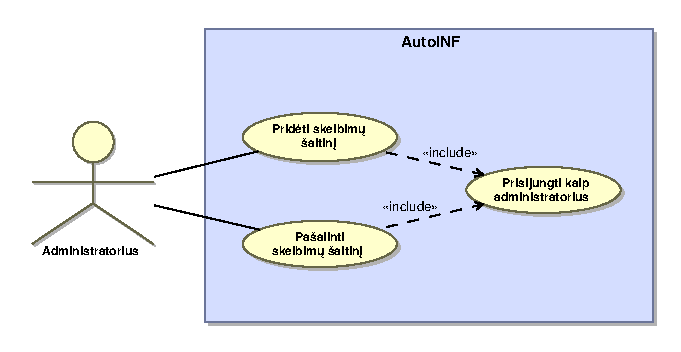
\includegraphics[width=0.7\textwidth]{TikslaiAdministratorius.eps}
			\caption{Sistemos užduočių diagrama iš administratoriaus perspektyvos\label{UseCaseAdmin}}
		\end{center}
	\end{figure}
	\pagebreak
	
	\subsubsection{Administratoriaus prisijungimo reikalavimai}
	\begin{enumerate}[labelindent=10pt,leftmargin=2.2cm]
		\item Administratoriaus prisijungimui taikomi visi reikalavimai, nurodyti \ref{LogInLabel} skyriuje.
		\item Sistema papildomai turi patikrinti, ar paskyra, prie kurios jungiamasi, yra administratoriaus paskyra.
	\end{enumerate}
		
		\begin{center}
		\captionof{table}{Pagrindinio lango scenarijus, kai administratorius yra prisijungęs\label{AdmindLoggedIn}}		
		\begin{tabular}{ | c | c | c | }
			\hline
			Žingsnis & Aktorius         & Veiklos apibūdinimas \\ \hline
			1        & Aplikacija       & \makecell{Aplikacija paprašo pasirinkti norimą veiksmą: \\ Pridėti skelbimų šaltinį \\ Pašalinti skelbimų šaltinį} \\ \hline
			2        & Administratorius & Administratorius pasirenka veiksmą \\ \hline
			3        & Aplikacija       & Aplikacija įvykdo pasirinktą veiksmą \\ \hline
		\end{tabular}
		\end{center}
		\bigskip
		
	\begin{enumerate}[resume,labelindent=10pt,leftmargin=2.2cm]
		\item Po sėkmingo administratoriaus prisijungimo sistema visada vykdo \ref{AdminViewSourcesScen} lentelėje pavaizduotą skelbimų šaltinių peržiūros funkciją.
	\end{enumerate}

		\begin{center}
		\captionof{table}{Administratoriaus skelbimų šaltinių peržiūros pagrindinis scenarijus\label{AdminViewSourcesScen}}
		\begin{tabular}{ | c | c | c | }
			\hline
			Žingsnis & Aktorius         & Veiklos apibūdinimas \\ \hline
			1        & Administratorius & Prisijungia \\ \hline
			2        & Aplikacija       & Siunčia užklausą į serverį \\ \hline
			3        & Serveris         & Siunčia užklausą į duomenų bazę \\ \hline
			4        & Duomenų bazė     & Grąžina skelbimų šaltinių sąrašą į serverį \\ \hline
			5        & Serveris         & Grąžina skelbimų šaltinių sąrašą į aplikaciją \\ \hline
			6        & Aplikacija       & Parodo skelbimų šaltinių sąrašą \\ \hline
		\end{tabular}
		\end{center}
		\pagebreak
	
	\begin{enumerate}[resume,labelindent=10pt,leftmargin=2.2cm]
		\item Nesėkmingo skelbimų šaltinių peržiūros atveju sistema į klaidas reaguoja pagal \ref{AdminViewSourcesScenExtra} lentelę.
	\end{enumerate}
	
		\begin{center}
		\captionof{table}{Administratoriaus skelbimų šaltinių peržiūros scenarijaus plėtiniai\label{AdminViewSourcesScenExtra}}		
		\begin{tabular}{ | c | c | c | }
			\hline
			Žingsnis & Sąlyga         & Veiklos apibūdinimas \\ \hline
			4a       & \makecell{Duomenų bazėje \\ nėra šaltinių} & \makecell{Duomenų bazė grąžina pranešimą, kad \\ skelbimų šaltinių nėra} \\ \hline
		\end{tabular}
		\end{center}
		\pagebreak
	
	\subsubsection{Administratoriaus skelbimų šaltinio pridėjimo reikalavimai}
	\begin{enumerate}[labelindent=10pt,leftmargin=2.2cm]
		\item Sėkmingo skelbimų šaltinio pridėjimo atveju sistema vykdo \ref{AdminAddSourceScen} lentelėje nurodytą veiksmų seką.
	\end{enumerate}
		
		\begin{center}
		\captionof{table}{Administratoriaus skelbimų šaltinio pridėjimo pagrindinis scenarijus\label{AdminAddSourceScen}}		
		\begin{tabular}{ | c | c | c | }
			\hline
			Žingsnis & Aktorius         & Veiklos apibūdinimas \\ \hline
			1        & Administratorius & \makecell{Suveda naujo skelbimų šaltinio duomenis ir \\ spaudžia mygtuką „Pridėti šaltinį“ } \\ \hline
			2        & Aplikacija       & Siunčia užklausą į serverį \\ \hline
			3        & Serveris         & Siunčia užklausą į duomenų bazę \\ \hline
			4        & Duomenų bazė     & \makecell{Prideda naują skelbimų šaltinį ir praneša \\ serveriui apie sėkmingą skelbimų šaltinio pridėjimą} \\ \hline
			5        & Serveris         & \makecell{Praneša aplikacijai apie sėkmingą skelbimų \\ šaltinio pridėjimą} \\ \hline
			6        & Aplikacija       & Atnaujina skelbimų šaltinių sąrašą \\ \hline
		\end{tabular}
		\end{center}
		\bigskip

	\begin{enumerate}[resume,labelindent=10pt,leftmargin=2.2cm]
		\item Nesėkmingo skelbimų šaltinio pridėjimo atveju sistema į klaidas reaguoja pagal \ref{AdminAddSourceScenExtra} lentelę.
	\end{enumerate}

		\begin{center}
		\captionof{table}{Administratoriaus skelbimų šaltinio pridėjimo scenarijaus plėtiniai\label{AdminAddSourceScenExtra}}		
		\begin{tabular}{ | c | c | c | }
			\hline
			Žingsnis & Sąlyga         & Veiklos apibūdinimas \\ \hline
			4a       & \makecell{Nepavyksta \\ pridėti šaltinio} & \makecell{Duomenų bazė grąžina pranešimą apie \\ nesėkmingą skelbimų šaltinio pridėjimą} \\ \hline
		\end{tabular}
		\end{center}
		\bigskip
		
	\begin{enumerate}[resume,labelindent=10pt,leftmargin=2.2cm]
		\item Skelbimų šaltinio pridėjimo funkcija administratoriui turi būti prieinama tik prieš tai sistemai atlikus skelbimų šaltinių peržiūros funkciją.
		\item Duomenų bazėje skelbimų šaltinis saugomas tokiu formatu:
		
			\begin{enumerate}[label=\theenumi.\arabic{enumii}]
				\item URL kodas,
				\item Skelbiamų transporto priemonių tipai (pvz., automobiliai, motociklai),
				\item Valstybės, kuriose skelbiamos visos šaltinio skelbimų transporto priemonės.
			\end{enumerate}
		 
	\end{enumerate}
	\pagebreak
	
	\subsubsection{Administratoriaus skelbimų šaltinio pašalinimo reikalavimai}
	\begin{enumerate}[labelindent=10pt,leftmargin=2.2cm]
		\item Sėkmingo skelbimų šaltinio pašalinimo atveju sistema vykdo \ref{AdminRemoveSourceScen} lentelėje nurodytą veiksmų seką.
	\end{enumerate}
		
		\begin{center}
		\captionof{table}{Administratoriaus skelbimų šaltinio pašalinimo pagrindinis scenarijus\label{AdminRemoveSourceScen}}		
		\begin{tabular}{ | c | c | c | }
			\hline
			Žingsnis & Aktorius         & Veiklos apibūdinimas \\ \hline
			1        & Administratorius & Pasirenka skelbimų šaltinio pašalinimą \\ \hline
			2        & Aplikacija       & Siunčia užklausą serveriui \\ \hline
			3        & Serveris         & Siunčia užklausą duomenų bazei \\ \hline
			4        & Duomenų bazė     & \makecell{Pašalina skelbimų šaltinį ir siunčia pranešimą \\ serveriui apie sėkmingai pašalintą skelbimų šaltinį} \\ \hline
			5        & Serveris         & \makecell{Siunčia pranešimą aplikacijai apie \\ sėkmingai pašalintą skelbimų sąrašą} \\ \hline
			6        & Aplikacija       & \makecell{Atnaujina skelbimų sąrašą ir laukia \\ tolimesnių administratoriaus veiksmų} \\ \hline
		\end{tabular}
		\end{center}
		\bigskip

	\begin{enumerate}[resume,labelindent=10pt,leftmargin=2.2cm]
		\item Nesėkmingo skelbimų šaltinio pašalinimo atveju sistema į klaidas reaguoja pagal \ref{AdminRemoveSourceScenExtra} lentelę.
	\end{enumerate}

		\begin{center}
		\captionof{table}{Administratoriaus skelbimų šaltinio šalinimo scenarijaus plėtiniai\label{AdminRemoveSourceScenExtra}}		
		\begin{tabular}{ | c | c | c | }
			\hline
			Žingsnis & Sąlyga         & Veiklos apibūdinimas \\ \hline
			4a       & \makecell{Nepavyksta \\ pašalinti šaltinio} & \makecell{Duomenų bazė grąžina pranešimą apie \\ nesėkmingą skelbimų šaltinio pašalinimą} \\ \hline
		\end{tabular}
		\end{center}
		\bigskip
		
	\begin{enumerate}[resume,labelindent=10pt,leftmargin=2.2cm]
		\item Skelbimų šaltinio pašalinimo funkcija administratoriui turi būti prieinama tik prieš tai sistemai atlikus skelbimų šaltinių peržiūros funkciją.
		\item Administratoriui pasirinkus skelbimų šaltinio šalinimą, sistema parodo naują langą, kuriame administratorius turi patvirtinti savo sprendimą.
	\end{enumerate}
	\pagebreak
	
	\renewcommand{\thesubsection}{NFR\arabic{subsection}}
	\renewcommand*{\theenumi}{\thesubsection.\arabic{enumi}}
	\renewcommand*{\theenumii}{\theenumi.\arabic{enumii}}
	\section*{Nefunkciniai reikalavimai}
	\addcontentsline{toc}{section}{Nefunkciniai reikalavimai}
	\setcounter{subsection}{0}
	
	\subsection{Vidinių interfeisų reikalavimai}
	\begin{enumerate}[labelindent=10pt,leftmargin=2.2cm]
		\item Sistema turi būti suprogramuota Java programavimo kalba.
		\item Sistema sukompiliuota laisvai platinamu standartiniu Java kompiliarotiumi.
		\item Sistema veikia Android aplinkoje, versijos pasirinkimas paliekamas programuotojų nuožiūrai.
		\item Programavimo aplinkos pasirinkimas paliekamas programuotojų nuožiūrai.
		\item Duomenims saugoti naudojama PostgreSQL duomenų bazė.
	\end{enumerate}	
	
	%\renewcommand*{\theenumi}{\thesubsubsection.\arabic{enumi}}
	%\renewcommand*{\theenumii}{\thesubsubsection.\theenumi.\arabic{enumii}}
	%\renewcommand*{\theenumiii}{\thesubsubsection.\theenumi.\theenumii.\arabic{enumiii}}
	%\subsection{Veikimo reikalavimai}
	%Šiame skyriuje aprašomi sistemos veikimo reikalavimai.
	
	\subsection{Tikslumo reikalavimai}
	\begin{enumerate}[labelindent=10pt,leftmargin=2.2cm]
		\item Skelbimo kaina atvaizduojama „double“ formatu 2 skačių po kablelio tikslumu ir nėra apvalinama.
		\item Duomenys apie valiutų kursus saugomi „double“ formatu. Skaičių kiekis po kablelio neribojamas.
	\end{enumerate}	
	
	\subsection{Patikimumo reikalavimai}
	\begin{enumerate}[labelindent=10pt,leftmargin=2.2cm]
		\item Įvykus bet kokiam sistemos sutrikimui, sistema, jei įmanoma, turi perkelti vartotoją į prieš tai atliktą žingsnį.
		\item Įvykus sutrikimui sistema neatskleidžia vidinių sutrikimo priežasčių vartotojui (nebent sutrikimas įvyko dėl jo kaltės). Visus sistemos lūžius ir to priežastis sistema saugo duomenų bazėje, prieinamoje tik savininkui ir administratoriams.
		\item Skelbimas vartotojo mėgstamiausiųjų sąraše atsiranda tik tada, kai jis pridedamas į duomenų bazę.
		\item Sistema nėra galima naudotis, kai atnaujinama sistemos duomenų bazė.
	\end{enumerate}	
	
	\subsection{Robastiškumo reikalavimai}
	\begin{enumerate}[labelindent=10pt,leftmargin=2.2cm]
		\item Visos klaidos yra saugomos sistemos duomenų bazėje, klaidų registre.
		\item Įvykus nedideliam sutrikimui (pvz., dingsta ryšys su duomenų baze; skelbimų šaltiniai nepasiekiami) sistema kartoja paskutinį veiksmą 30 s. Neatsistačius funkcionalumui sistema išsaugo klaidos priežastį duomenų bazėje, atsiprašo vartotojo už nepatogumus ir prašo vartotojo pabandyti naudotis sistema vėliau.
		\item Įvykus rimtam sutrikimui (pvz., atnaujintas skelbimų puslapio HTML kodas; pasikeičia skelbimų nuskaitymo būdas, todėl nebeįmanoma gauti skelbimų informacijos), sistema turi gebėti išimti puslapį iš pasirinkimo galimybių ir užregistruoti veiksmą duomenų bazėje.
		\item Po sistemos sutrikimo tikėtinas atsistatymo laikas yra laikas, reikalingas sistemos perkrovimui.
		\item Sutrikus infrastruktūrai (pvz., duomenų bazei) sistema pradeda veikti iš karto, kai infrastruktūra yra sutvarkyta.
	\end{enumerate}	
	
	\subsection{Našumo reikalavimai}
	\begin{enumerate}[labelindent=10pt,leftmargin=2.2cm]
		\item Sistema vos pradėjusi paiešką turi pranešti vartotojui, kad priėmė paieškos duomenis ir kad paieška yra vykdoma.
		\item Sistema turi parodyti pirmąjį užklausos puslapį ne lėčiau kaip per 10 s.
		\item Sistema į vartotojo įvestį turi sureguoti ne lėčiau kaip per 0,5 s.
		\item Užklausų skaičius, kurį maksimaliai be vėlavimo gali atlikti serveris, yra 10 000 per sekundę (nebent sistemos savininko infrastruktūra nėra pakankamai pajėgi).
	\end{enumerate}
	
	\pagebreak
	\renewcommand{\thesubsection}{IR\arabic{subsection}}
	%\renewcommand*{\theenumi}{IR\arabic{enumi}}
	%\renewcommand*{\theenumii}{\theenumi.\arabic{enumii}}
	\section*{Interfeiso reikalavimai}	
	\addcontentsline{toc}{section}{Interfeiso reikalavimai}
	\setcounter{subsection}{0}	
	\subsection{Bendri reikalavimai}	
	\begin{enumerate}[labelindent=10pt,leftmargin=2.2cm]
		\item Originali valiuta automatiškai vaizduojama eurais, bet vartotojas gali pasirinkti, kurią valiutą iš pagrindinių (pagrindinės valiutos pasirenkamos programuotojų atžvilgiu, bet nemažiau kaip 3, iš kurių viena - euras) rodyti.
		\item\label{MainWindowDisplayReq} Pagrindinis langas, kuris atvaizduojamas įjungus programą, yra paieškos langas.
		\item\label{AdParts} Visi skelbimai sąraše atvaizduojami formatu, kurio pagrindinės dalys yra:
		
		\begin{enumerate}[label=\theenumi.\arabic{enumii}]
			\item Pagrindinė skelbimo nuotrauka,
			\item Transporto priemonės markė,
			\item Transporto priemonės modelis,
			\item Kuro tipas,
			\item Variklio litražas,
			\item Kėbulo tipas,
			\item Valstybė,
			\item Metai,
			\item Kaina.
		\end{enumerate}
		
		\item Paieškos lange turi būti leidžiama pasirinkti skelbimo pagrindinių dalių (transporto priemonės markės ir modelio) paieškos filtrus, tačiau galima ir detalesnė paieška.
		\item Detalesnei paieškai turi būti atskiras langas su platesne pasirinkimų specifikacija.
		\item Privalomi laukai turi būti pažymėti „ * “ simboliu
		\item Laukai „Kaina“ ir „Metai“ turi būti leidžiami pasirinkti tipu „Nuo-Iki“, tačiau veikimas privalomas tiek neužpildžius nė vieno iš šių laukų, tiek detalizavus tik „Nuo“, tiek detalizavus tik „Iki“, tiek detalizavus abu.
		\item Paieškos tipai (mažiausiai 3, pvz., automobiliai, motociklai, elektromobiliai) turi būti lengvai keičiami skirtukais („Tabs“) pagrindiniame paieškos lange.
		\item Viename paieškos rezultatų lange gali būti ne daugiau kaip 20 skelbimų. Likę (jei jų yra) perkeliami į kitus puslapius.
		\item Po 10 skelbimų (jei tiek nėra - sąrašo pabaigoje) turi būti išskirta vieta reklamai. Dydis pasirenkamas programuotojo nuožiūra, tačiau nedidesnis nei skelbimo dydis.
		\item Paieškos rezultatų lango viršuje turi būti rodomi vartotojo įvesti paieškos kriterijai.
		\item Sistemoje turi būti įdiegta galimybė bet kuriame jos etape grįžti į pagrindinį paieškos langą ir, jei vartotojas yra prisijungęs, į mėgstamiausių skelbimų sąrašo langą (jei vartotojas nėra prisijungęs - į prisijungimo langą). Siūlomas sprendimas - įrankių juosta virš visų langų.
		\item Įrankių juostos mygtukai „Mėgstamiausių sąrašas“, „Prisijungimas“ ir „Registracija“ turi būtinai būti matomi. Kiti, papildomi mygtukai (pvz., „Nustatymai“) gali būti pasislėpę po perpildančiu („Overflow“) sąrašu.
		\item Visi skelbimai turi turėti aiškų mygtuką, kuris leidžia skelbimą pridėti prie mėgstamiausių sąrašo.
		\item Mėgstamiausių skelbimų sąrašo visi skelbimai turi turėti aiškų mygtuką, kuris leidžia skelbimą pašalinti iš mėgstamiausių sąrašo.
		\item Vartotojui prisijungus registracijos mygtuko nebelieka.
		\item Langas, vaizduojamas prisjungus administratoriui, yra skelbimų šaltinių peržiūros langas. 
	\end{enumerate}
		
	\subsection{Ergonominiai reikalavimai}
	\begin{enumerate}[labelindent=10pt,leftmargin=2.2cm]
		\item Šriftų dydis pagrindiniame lange ne mažesnis nei 20 pt, skelbimo formate - ne mažesnis nei 10 pt.
		\item Tarpai tarp eilučių turi būti tokie, kad eilutės nesiliestų viena su kita.
		\item Atsižvelgiant į \ref{MainWindowDisplayReq} punktą vartotojui nedetalizavus paieškos pagrindiniam sistemos veiksmui (paieškai) atlikti užtenka 1 veiksmo - paspausti paieškos mygtuką, kuris turi būti pagrindiniame lange ir turi būti didelis ir gerai matomas.
		%\item Sistema neturi būti pritaikyta neįgaliesiems.
	\end{enumerate}
	\pagebreak
	
	\section*{Rezultatai}	
	\addcontentsline{toc}{section}{Rezultatai}
	Šiame laboratoriniame darbe yra atskleidžiami sistemos reikalavimai, kurie išskaidyti į funkcinius, nefunkcinius ir interfeiso reikalavimus. Funkciniuose reikalavimuose išvardijamos esminės sistemos funkcijos ir aprašomas vartotojo bei administratoriaus užduočių įgyvendinimas. Nefunkciniuose reikalavimuose yra apibrėžiamos neesminės sistemos funkcijos, įprasminančios pagrindines sistemos funkcijas. Interfeiso reikalavimai parodo, kaip sistemos atliekamos funkcijos turi būti pateiktos vartotojui, kad būtų patogu naudotis sistema.
	\pagebreak
	
	\section*{Išvados}	
	\addcontentsline{toc}{section}{Išvados}
	Šis reikalavimų dokumentas užtikrina, kad programuotojai vienareikšmiškai supras, kaip sistema turi atrodyti ir veikti ir tuo pačiu užtikrins, kad šia sistema bus galima lengvai pasinaudoti bet kokiam vartotojui.
\end{document}
